\section{Program structure}
\label{qoala:sec:app:program_structure}
This section provides details about the structure and contents of Qoala programs as described in Section~\ref{qoala:sec:program_structure}.


\subsection{Program representation and components}
A Qoala program is represented in human-readable text format.
This allows one to directly write Qoala programs, although our vision is that programmers write their code in a higher-level language, and that a compiler translates this into a Qoala program.

In the main text, some parts of example programs were omitted for brevity.
In Figure~\ref{fig:app:example_full_program} we show an example of a full Qoala program.

A Qoala program encompasses both classical and quantum code.
These different code segments are put into different sections in the program.
The host section contains QoalaHost code which is to be run on the CPS.
The NetQASM section contains local routines (containing NetQASM instructions) which are meant to be run on the QPS.
The request section contains specifications of requests for remote entanglement generation, to be handled by the QPS.
Furthermore, there is a meta section which defines global information about the program.
Each of these sections is explained in more detail below.

In all of the sections in a Qoala program, values may be replaced by a \textbf{template}.
A template represents a value that is not defined for the program, but is filled in at program instantiation. For example, a QKD program might have a request object in its request section containing the entry \texttt{num\_pairs: {N}}, where \texttt{{N}} is a template. This construction allows one to instantiate the same program with different values for \texttt{N}, and it is hence not needed to define separate programs for each different number of pairs to generate in the QKD program.

\subsection{Program Meta}
Program metadata contains:

\begin{itemize}
    \item \textbf{Name}: The name of this program.
    \item \textbf{Parameters}: Global arguments to this program. These arguments may be used as templates (see above) in the program. Examples may be the name of a remote node, or the number of EPR pairs to generate.
    \item \textbf{Classical Sockets}: A mapping from IDs to remote node names. The IDs are local identifiers that can be used by Host code to distinguish different classical sockets.
    \item \textbf{EPR Sockets}: A mapping from IDs to remote node names. The IDs are local identifiers that can be used by Host code to distinguish different EPR sockets.
\end{itemize}


\begin{figure*}[ht]
    \centering
    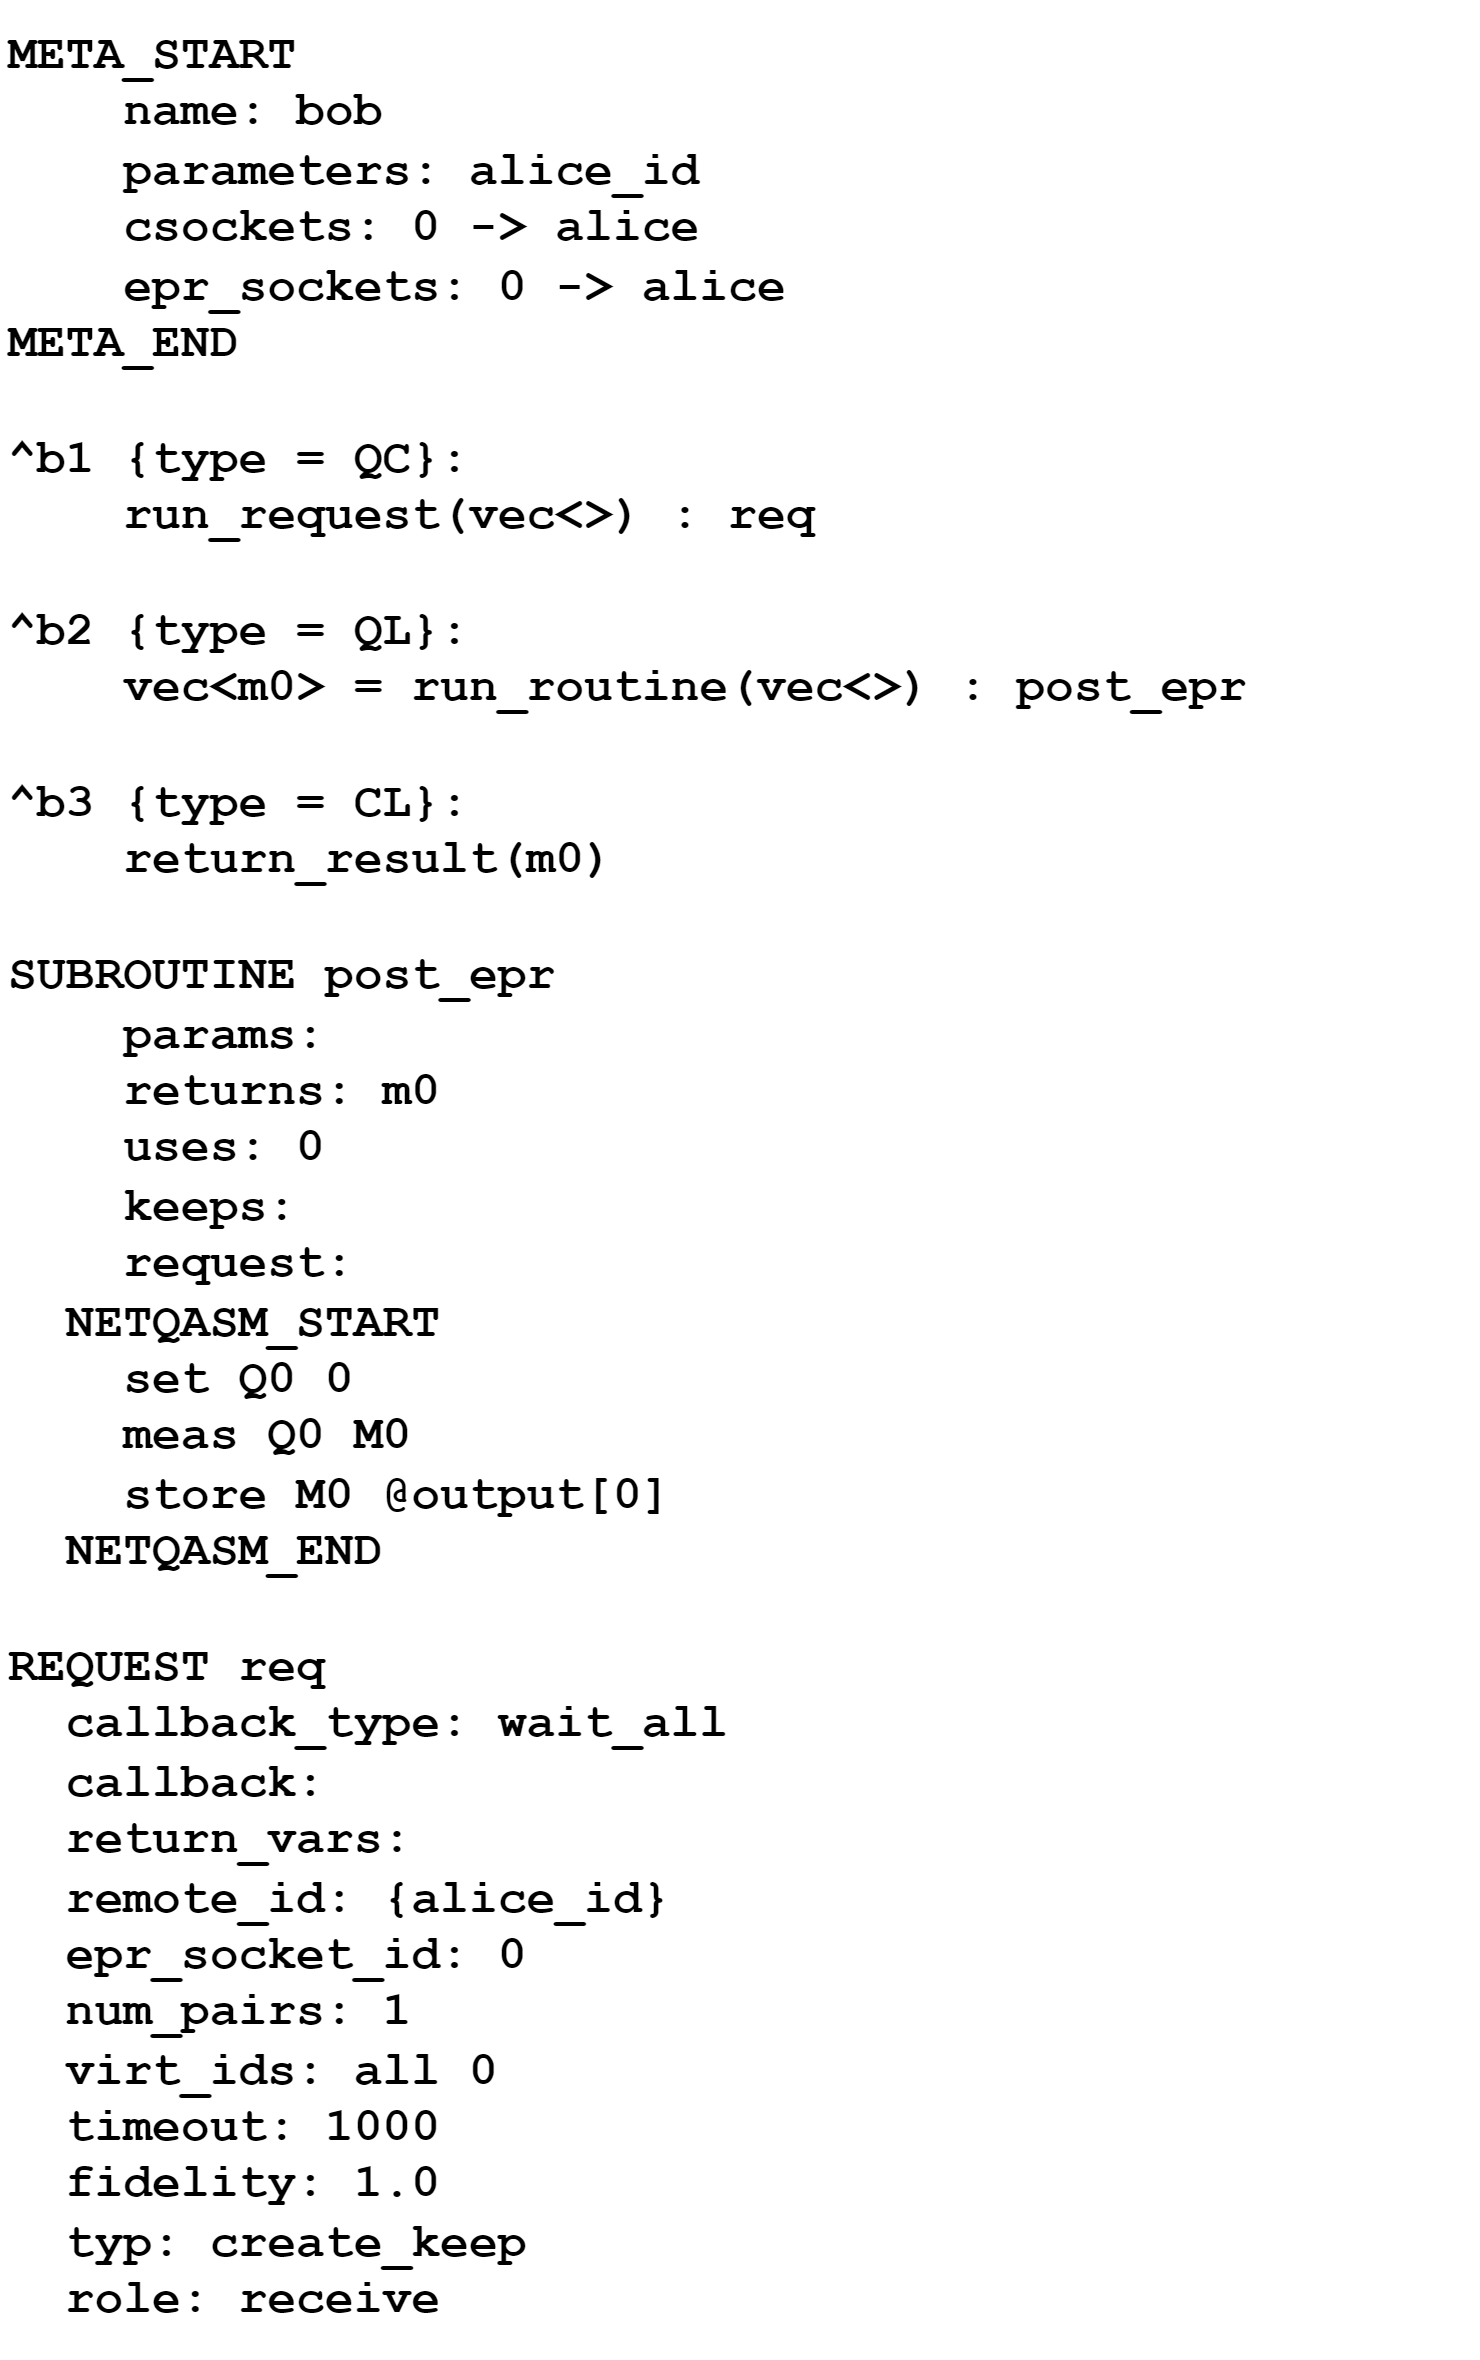
\includegraphics[scale=1.0]{figures/qoala/appendix_example_full_program.png}
    \caption{Example Qoala program which creates an EPR pair with remote program Alice, measures the local qubit, and returns the classical outcome value.
    \textit{Meta section.} The meta section defines the name of this program, the global arguments (input values, in this case: the node ID of the Alice program),
    the classical sockets used (mapping local socket ID to the name of the remote node, and the EPR sockets used (also mapping local socket ID to remote node names)).
    \textit{Host section.} This example host section consists of three blocks (\texttt{b1, b2, b3}). \texttt{b1} calls request routine \texttt{req} (no result values).
    \texttt{b2} calls local routine \texttt{post\_epr}, resulting in a classical vector with one value (\texttt{m0}).
    \texttt{b3} returns \texttt{m0} as the result of this program.
    \textit{Local routines section.} Consists of a single local routine called \texttt{post\_epr}.
    It requires the virtual qubit (see Section~\ref{qoala:sec:app:runtime_environment}) with ID 0 to be allocated, and acts on this qubit.
    Upon finishing the local routine, this qubit is not in use anymore (the \texttt{keeps} entry is empty).
    The NetQASM code represents measuring the qubit, and then storing the result (in register \texttt{M0}) to the \texttt{@output} array (see Section~\ref{qoala:sec:app:runtime_environment}), which is in shared memory and can be accessed by host code by the name \texttt{m0}.
    \textit{Request routines section.} Consists of a single request routine called \texttt{req}.
    It represents a request to the network stack for generating a single entangled pair (\texttt{num\_pairs} is 1), which is kept in memory (\texttt{typ: create\_keep}; not measured immediately).
    This program acts as a `receiver' for entanglement generation (\texttt{role} attribute), which breaks symmetry in the entanglement generation process (the remote Alice program will have \texttt{role: sender}). Symmetry breaking is needed for the network stack to organize the entanglement generation.
    No callbacks are used, and all qubits (in this case: one) are stored in virtual qubit 0.
    }
    \label{fig:app:example_full_program}
\end{figure*}

\subsection{Host section}
The host section contains code the be executed by the CPS.
It consists of both local processing (like calculation and conditional logic), and
communication (sending and receiving classical messages to and from other nodes in the network).

The language in which host code is represented is called QoalaHost.
This is a low-level instruction set with well-defined semantics and types,
and is meant to be executed by a virtual machine or interpreter.
One can also imagine QoalaHost code to be translated (either ahead-of-time or at just-in-time) to native CPS code, such as x86 or ARM. However, for the sake of simplicity and of implementation independence, we treat here only the QoalaHost language and its semantics itself.

The QoalaHost (QH) language was designed to resemble intermediate representations as found in LLVM~\cite{lattner2004llvm} and MLIR~\cite{lattner2021mlir},
such that integration with future compilers is accessible.
Specifically, one may imagine a compiler that uses MLIR for its intermediate representation (IR).
When this compiler then produces the host code of the program, the translation of its own IR to QoalaHost code should be straightforward.

\textbf{Blocks.} 
The Host section consists of a list of blocks.
A block consists of a block metadata and a list of QH instructions.

The block metadata contains the following entries:
\begin{itemize}
\item \textbf{Name}: The name of this block. Host code can refer to this name in QH branch instructions.
\item \textbf{Type}: one of CL, CC, QL or QC (see below).
\item \textbf{Deadlines}: Deadlines relative to other blocks.
The deadlines are specified in terms of EHI arguments. Upon program instantiation, concrete values are filled in based on the actual EHI value.
\item \textbf{Time hints}: Duration estimate of executing the block.
The estimates are specified in terms of EHI arguments. Upon program instantiation, concrete values are filled in based on the actual EHI value.
\end{itemize}


\subsection{Block types}
Blocks are categorized into the following four types:
\begin{itemize}
\item \textbf{CL}: Classical Local. The block contains only instructions that are classical, local and only involve the CPS
\item \textbf{CC}: Classical Communication. CPS-only instructions, but starts with a `receive message` instruction.
\item \textbf{QL}: Quantum Local. The block contains calls to local routines.
\item \textbf{QC}: Quantum Communication. The block contains calls to request routines.
\end{itemize}


\textbf{QoalaHost Language.}
The QH Language describes a fixed set of QH instructions as well as QH Variable types.
Host code is represented as blocks containing QH instructions.
These instructions may be directly interpreted by a processor or OS.

All basic values are 32-bit signed integers (i32) or floating point values (f32).
A variable in Host code can either be
\begin{itemize}
\item singleton variable, holding one basic value. Has a single name. E.g. \texttt{x}
\item vector, holding an arbitrary number of basic values. Has a single name. E.g. \texttt{x<>}
\end{itemize}

The QH Language allows for expressing multiple variables in a single expression, called a \textit{tuple}.
A tuple holds a fixed number of basic values. E.g. \texttt{tuple<x, y, z>}.

\textbf{Local Memory.}
Host code is assumed to have access to a local memory space that is logically organized as a mapping of \textit{names} to \textit{values}.
For example, the local memory may at some point during execution contain the following items:

\begin{lstlisting}
"var_x" -> 3
"my_vec" -> <1, 2, 5>
\end{lstlisting}


\textbf{Shared Memory.}
The QH Language does not allow direct access to shared memory.
Only variables from the local memory can be used.
When calling and getting results from Local Routines (LRs) and Request Routines (RRs), values are automatically
moved from local memory to shared memory. 
Shared memory is discussed in more detail in Appendix~\ref{qoala:sec:app:shared_memory}.

\subsubsection{Block format}

A block has the following format:
\begin{lstlisting}
^#name {type = #type}:
    <list of QH instructions>
\end{lstlisting}

Example:
\begin{lstlisting}
^b0 {type = CL}:
    x = assign() : 3
    return_result(x)
\end{lstlisting}


\begin{figure*}
    \centering
    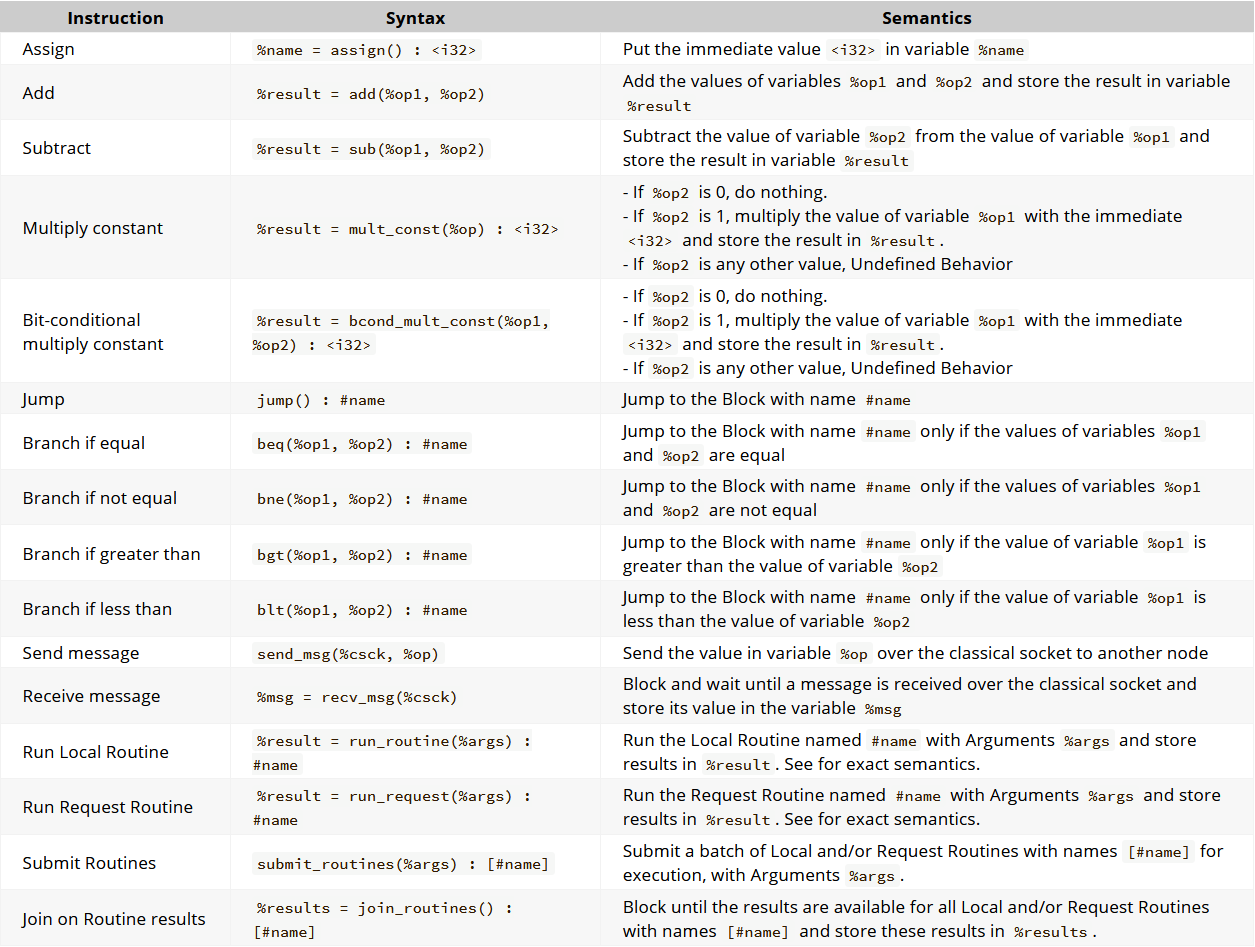
\includegraphics[scale=0.35]{figures/qoala/qh_table.png}
    \caption{Overview of all host code (QoalaHost) instructions, their syntax and their semantics.}
    \label{fig:app:qh_table}
\end{figure*}

\subsubsection{QH instructions}
A full list of QoalaHost instructions is given in Table~\ref{fig:app:qh_table}.


\subsection{NetQASM section}
\label{qoala:sec:app:netqasm}
The NetQASM section consists of a list of local routines that are to be executed on the QPS.
A local routine is only executed when it is called by host code using the \texttt{run\_routine} instruction. A local routine may be run multiple times, again depending on the host code.

The instructions of a local routine are represented using the NetQASM 2.0 format.
This is an updated format compared to NetQASM 1.0 as presented in~\cite{dahlberg2022netqasm}.

\begin{figure*}
    \centering
    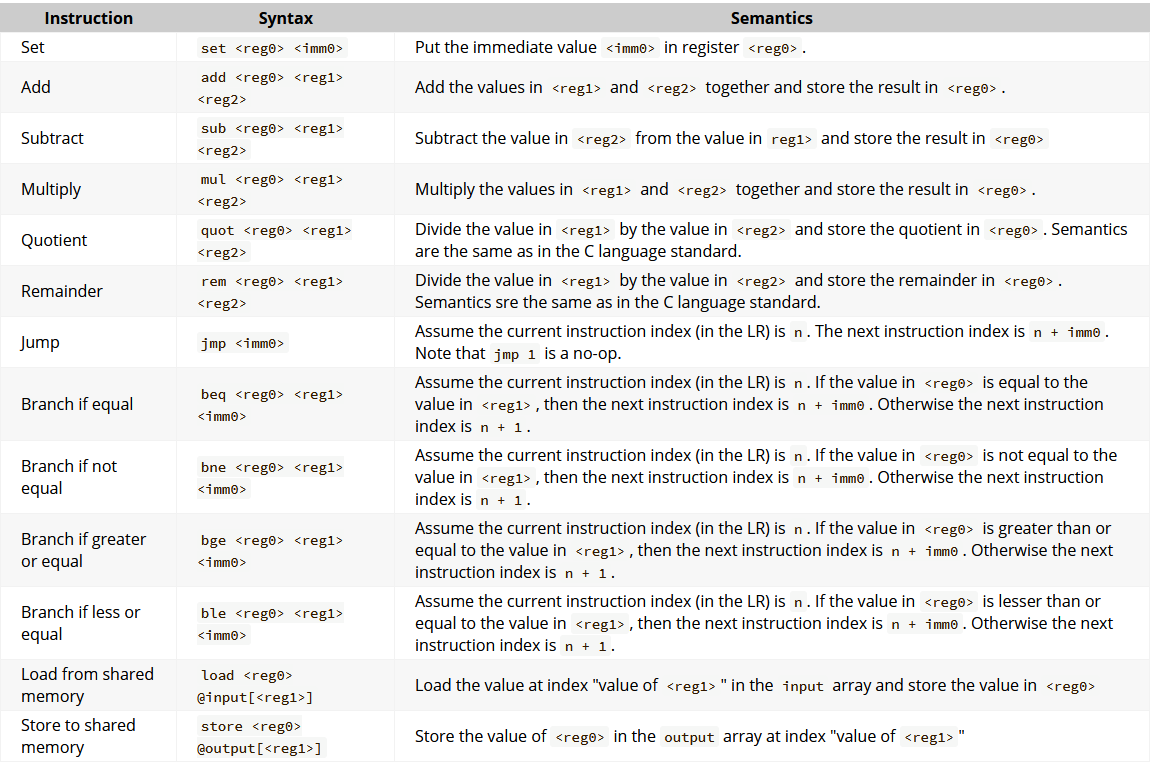
\includegraphics[scale=0.4]{figures/qoala/netqasm_table.png}
    \caption{Overview of all NetQASM classical instructions, their syntax and their semantics.
    Quantum instructions depend on the particular flavour~\cite{dahlberg2022netqasm} that is being used.}
    \label{fig:app:netqasm_table}
\end{figure*}


\textbf{NetQASM values.}
All values are 32-bit signed integers. Floating-point values are not supported. Angles for qubit rotations must be expressed as discrete values.
Booleans are represented as follows: \texttt{true} is the 32-bit 0 value, \texttt{false} is the 32-bit 1 value. Any other 32-bit value is not a valid boolean.
The reason for keeping the different types limited is to keep the QPS implementation simple.


\textbf{NetQASM Local Memory}
The QPS is expected to have a local memory (only accessible by the QPS itself) consisting of 64 32-bit registers:
\begin{itemize}
\item 16 \textbf{R} registers: \texttt{R0} to \texttt{R15}
\item 16 \textbf{C} registers: \texttt{C0} to \texttt{C15}
\item 16 \textbf{M} registers: \texttt{M0} to \texttt{M15}
\item 16 \textbf{Q} registers: \texttt{Q0} to \texttt{Q15}
\end{itemize}

The four groups of registers are not inherently different. A compiler producing NetQASM code may use a certain group only for certain values, but this is not mandatory.

\textbf{Shared Memory}
See Appendix~\ref{qoala:sec:app:shared_memory} for more information about Shared Memory and arrays.
The QPS is expected to have access to Shared Memory (accessible by both the CPS and QPS).
Two shared memory Arrays are available:
\begin{itemize}
\item an \texttt{@input} array, containing the LR input variables
\item an \texttt{@output} array, with space to write the LR results to
\end{itemize}

The length of the \texttt{@input} array is equal to the number of LR parameters.
The length of the \texttt{@output} array is equal to the number of LR return variables.

\begin{itemize}
\item The \texttt{@input} and \texttt{@output} arrays are the only arrays accessible from within the LR.
\item The QPS can \textbf{only read} from the \texttt{@input} array (see \texttt{load} instruction below).
\item The QPS can \textbf{only write} to the \texttt{@output} array (see \texttt{store} instruction below).
\end{itemize}

\textbf{NetQASM Instruction}
Each instruction consists of the instruction type followed by a list of operands.
The text form of an instruction is:

\begin{lstlisting}
instr_name  op0 op1 ... opn
\end{lstlisting}

where the number of operands can be 0 or more (no limit).

A list of all NetQASM 2.0 instructions can be found in Table~\ref{fig:app:netqasm_table}.

These instructions can be classified as:
\begin{itemize}
\item shared memory access: \texttt{load} for reading LR inputs, \texttt{store} for writing LR results
\item classical logic and control-flow: like \texttt{set} , \texttt{add}, or \texttt{jmp}
\item quantum operations: gates from a specific flavour~\cite{dahlberg2022netqasm}
\end{itemize}

NetQASM instructions representing quantum operations are either \textit{core instructions} or \textit{flavour-specific} instructions.
Core instructions are quantum hardware independent and are expected to be compatible with any QPS implementation. On top of the core instructions, flavour-specific instructions may be added and supported by a specific QPS implementation. For example, a QPS that controls an NV-centre may support NetQASM instructions of the NV flavour, which contain gate operations only available on this particular quantum hardware. Which NetQASM instructions are supported by the QPS is exposed to higher layers (including a compiler) as part of the EHI (see Appendix~\ref{qoala:sec:app:ehi}). Using this information, a compiler may produce optimized NetQASM code using the flavour-specific NetQASM instructions.


Note that NetQASM 2.0 \textbf{does not} contain (in contrast to NetQASM 1.0~\cite{dahlberg2022netqasm}):
\begin{itemize}
\item Allocation instruction (\texttt{qalloc} in NetQASM 1.0): The memory manager allocates virtual qubits based on the LR header information. Note that qubit allocation is different from \textit{qubit initialization} (\texttt{init} instruction).
\item Instructions for EPR generation: This is handled by request routines.
\item Waiting instructions: Waiting is handled by the scheduler choosing which tasks to execute when.
\end{itemize}

\textbf{Local Routine}
A Local Routine (LR) represents a block of local program operations that are executed on the QPS. An LR is:
\begin{itemize}
\item local: there is no interaction whatsoever with external nodes or controllers
\item atomic: execution of an LR cannot be pre-empted; when the QPS start executing an LR, it will not do anything else until the LR has finished (unless an abort happens)
\end{itemize}

An LR consists of a \textit{header} and a \textit{body}. The header contains metadata such as the resource usage of the LR, and its input/output interface. The body contains the actual instructions in the form of NetQASM code.


\textbf{Arguments and Returns.}
An LR may have zero or more \textit{arguments}: values that are provided to the LR only at runtime.
They can be seen as inputs or parameters to the LR.
These values appear in the \texttt{@input} array in shared memory, and are put there by the CPS.

An LR may also have zero or more \texttt{returns}: values that are provided by the LR only at runtime.
They can be seen as outputs or results of the LR.
These values must be written to the \texttt{@output} array in shared memory, and can then be used by the CPS.

Arguments and returns are always 32-bit signed integers. There is no limit to the number of arguments and returns an LR may have.

\textbf{Local routine header.}
A Local routine (LR) header contains the following entries:
\begin{itemize}
\item \textbf{Name}: The name of this LR. Host code refers to this name in a \texttt{run\_routine} QoalaHost instruction.
\item \textbf{Uses}: A list of virtual qubits IDs. These refer to all virtual qubits that are used by this LR. At runtime, the memory manager makes sure that these virtual qubits are allocated before execution of the LR starts. (They may already have been allocated earlier; alternatively the memory manager allocates them just before the LR starts.)
\item \textbf{Keeps}: A list of virtual qubit IDs. These refer to all virtual qubits that should \textit{remain allocated} after finishing the LR. (They may e.g. be used in subsequent LRs.)
\item \textbf{Args}: A list of names for the arguments of the LR. They are in the same order as how their values are accessible from the \texttt{@input} Array.
\item \textbf{Returns}: A list of names for the returns of the LR. They are in the same order as how their values are put into the \texttt{@output} Array.
\end{itemize}

\textbf{Quantum memory usage annotations.}
The LR header indicates which virtual qubits are used and freed by the LR. This makes it possible for the scheduler to decide which \texttt{LocalRoutine} task it may schedule when. For more information, see section Appendix~\ref{qoala:sec:app:scheduling_execution} on scheduling.
The following listing provides an example:

\begin{lstlisting}
SUBROUTINE subrt1
    uses: 0, 1
    keeps: 0
    returns: m0
    <rest omitted>
  NETQASM_START
    set Q0 0
    set Q1 1
    init Q0
    init Q1
    cnot Q0 Q1
    meas Q1 M1
    store M1 @output[0]
  NETQASM_END
\end{lstlisting}
This local routine initializes virtual qubits 0 and 1 and then applies a CNOT gate on them.
It measures qubit 1 and stores the output in the \texttt{@output} array which can then be accesses by host code using the name \texttt{m0}.
Using the metadata, a scheduler knows the following information even before executing this LR: virtual qubits 0 and 1 need to be free before this LR can run, and after running the LR, qubit 1 is free (again) but qubit 0 remains occupied.

It is the responsibility of the compiler to make sure that the use and free values correspond to the actual NetQASM code.


\subsection{Request section}
The callback (which is an LR) can have zero or more arguments (just like standard LRs). The runtime values of these arguments are provided by the QPS directly.
A Request Routine (RR) may have zero or more returns: outputs or results of the entire RR. The only allowed results at this moment are measurement outcomes in case of Measure Directly requests.
RR callbacks can have (just like standard LRs) zero or more returns.


\textbf{Request routine header}
A Request routine (RR) header contains the following entries:
\begin{itemize}
\item \textbf{Name}: The name of this RR. Host code refers to this name in a \texttt{run\_request}.
\item \textbf{Returns}: A list of names for the returns of the RR. Since the returns can only be measurement outcomes, these names are either (1) the name of a single QoalaHost vector variable which will hold all outcomes, or (2) a list of names for each individual outcome stored in its own QoalaHost int variable.
\item \textbf{Callback type}: Either \texttt{sequential} or \texttt{wait\_all}. Sequential means that the callback of this RR is executed for each generated pair, before the next pair is generated. Wait-all means that the callback is only executed once, namely when all pairs have been generated.
\item \textbf{Callback}: The name of the LR that acts as the callback for this RR. Can be empty (no callback is used).
\end{itemize}


\textbf{Request Parameters}
\begin{itemize}
\item \textbf{Remote ID}: The node ID of the remote node with which to generate entanglement.
\item \textbf{EPR Socket ID}: The ID of the EPR Socket to use.
\item \textbf{Number of pairs}: The number of entangled pair to generate.
\item \textbf{Virtual IDs}: A specification of the virtual IDs to assign to the entangled qubits. This may be in one of three formats:
\begin{itemize}
  \item \texttt{all <N>}: all qubits get virtual ID \texttt{<N>}. This might be used when a sequential callback is used that measures the qubit immediately after generating; thereby freeing up virtual ID \texttt{<N>} immediately for the next pair
  \item \texttt{increment <N>}: the first generated qubit gets ID \texttt{<N>}, the next \texttt{<N> + 1}, etc.
  \item \texttt{custom <N1, N2, ...>}: a custom list of IDs that should have the same length as the number of pairs
\end{itemize}
\item \textbf{Fidelity}: The desired fidelity \texttt{F} of the generated pairs.
If this request routine is for multiple pairs and the callback type is \texttt{wait\_all}, this value is used to specify that all pairs, after they have all been created, should have fidelity at least \texttt{F}. (How this is realized, which may involve multiple retries, is up to the network stack implementation in the QPS.)
\item \textbf{Type}: Create and Keep (\texttt{create\_keep}), Measure Directly (\texttt{measure\_directly}), or Remote State Preparation (\texttt{rsp}) \cite{dahlberg2019link}.
\item \textbf{Role}: \texttt{create} or \texttt{receive}. These roles are used to break symmetry between two nodes participating in entanglement generation (they should always have different roles). The `create' node is the initiating one.

\end{itemize}




